
\section{Designing for Simulated Roleplay}

\textbf{\textit{Formative Testing}} With 5 experienced counselors from the online peer support platform~\citeauthor{7cupswebsite}, we conducted 90 minute testing sessions to discover their needs for constructing a virtual patient with our human-LLM interaction tool. In the session, a counselor constructed two virtual patient bots, where the first bot was based on a common scenario. Counselors all used the principle elicitation features to interactively shape the virtual patient in a median 40 minutes time ($min = 30$ minutes; $max = 75$ minutes). We also observe a diversity of principles created for virtual patients made based on a common scenario and for one's based on a counselor's own personal experiences. This validates the need for tools that supports customization of the virtual patient's behaviors according to principles defined by counselors. A more detailed set of themes from these formative tests is given in Appendix~\ref{sec:appendix_formative}.

In terms of tool experience, counselors liked the multiple pathways they could give feedback on behaviors and enjoyed the ability to add principles, rewind the conversation, and see changes in the generated responses. Scores on a tool usage questionnaire were in slight to strong agreement, with raw scores in Table~\ref{tab:tooluse-formative} in Appendix~\ref{sec:appendix_formative}.  While early prototypes using GPT3.5 exhibited periodic issues with principle adherence and response repetition, our later prototypes showed a qualitatively reduced frequency of these issues by using a GPT-4 powered dialogue-simulation. With a stronger base LLM system, this motivated us systematically analyze the virtual patients' response generation capabilities, which we detail in the next section.  
% Between test sessions, we improved the tool based on software bugs and usability issues that arose. Our later prototypes used a GPT-4 powered dialogue-simulation, as we observed frequent issues with principle adherence and response repetition when using a dialogue-simulation powered by the GPT-3.5 model.  

\begin{figure*}[t]
    \centering
    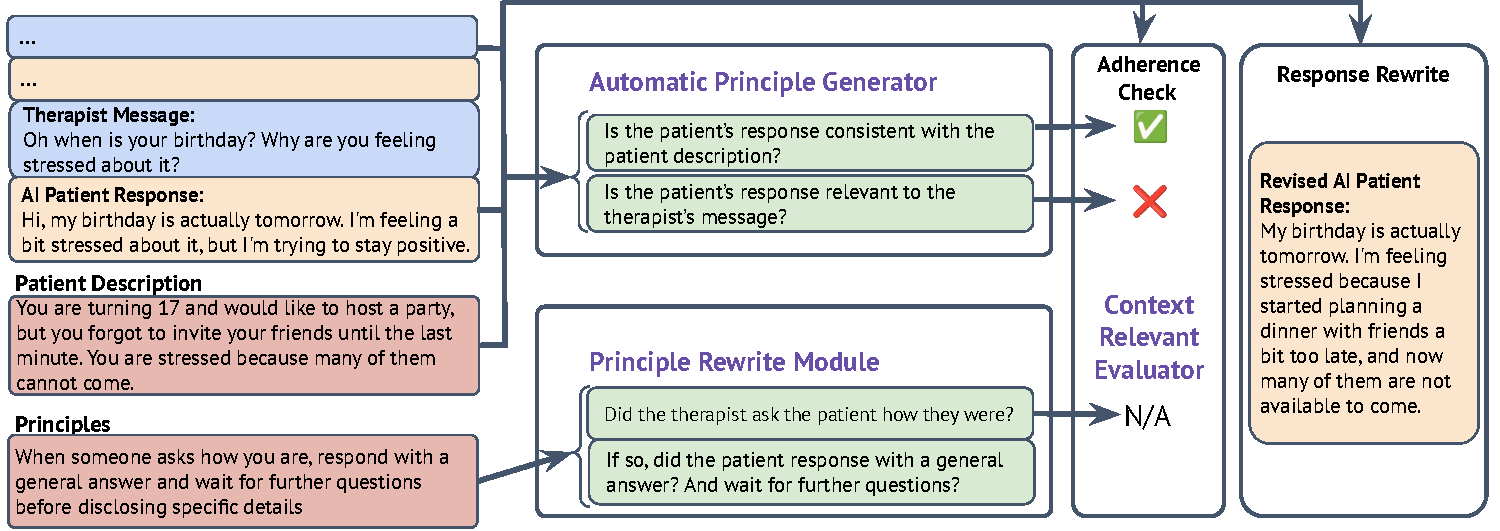
\includegraphics[width=\textwidth]{figures/principle-adherence-module.pdf}
    \caption{LLM Program for more reliable constitution principle following. \ryan{Could we simplify the diagram even further (still a lot of text). (1) pick a representative example trace; (2) label key things that we should notice; (3) highlight where your method comes through.} It is capable of (1) assessing which explicit principles and implicit conventions are relevant to the dialogue context; (2) decomposing simple and composite principles into a set of yes/no principles; (3) answering principle-adherence questions with justifications (not shown); and (4) revising the response to adhere to all the principles.}
    \label{fig:agent-critique-improve}
\end{figure*}

\subsection{Analysis of Base Principle Following Capabilities} % Principle Following Test % Testing GPT's zero-shot ability to generate dialogue responses given the principles 
We aim to determine how often directly prompting GPT-4 produces a less satisfying response with respect to the principles.  Testing this once the virtual patient is created with fixed principles allows us to more realistically simulate how a novice peer supporter might use a virtual patient.

\textit{\textbf{Procedure:}} We selected 4 virtual patients that were created in the design sessions by different counselors. For virtual patients that had multiple principles generated for a single feedback (due to UI bug which allowed doubly-saving their feedback), we cleaned up these duplicated. Four co-authors had practice conversations with each of the four virtual patients, resulting in a total of 16 conversations. Each response in the conversations was rated on a 5 point likert scale (5 = Completely, 1 = Not at all) on how satisfying the generated response was with respect to the principles and conversation context. From the 16 completed convesations, the mean number of responses was 17.25, with a minimum of 12 and maximum of 22. In total, 276 responses were given satisfaction ratings. % \ryan{TODO: Describe process for reaching annotator agreement, and deciding rules for dialogue context, or interpreting the spirit of the principles}

\textit{\textbf{Results:}} 80\% of generated responses (221/276) were rated as completely or mostly satisfying given the principles and conversation context. Conversely, 20\% (55/276) of responses generated by directly prompting the GPT model were rated as moderately, slightly, or not at all satisfying.  
This result highlights that directly prompting the most capable LLM (\lstinline{gpt-4-turbo-1106-preview} holds the \#1 rank on the lmsys leaderboard at the time of writing) still produces responses in which some principles are not being followed, or in which responses are awkward given the dialogue context.  We break down these less than satisfactory responses into several categories.

% \ryan{TODO: In the appendix, we could show a table of the ratings, broken down by virtual patients. Each virtual patient was complex, but the very complex virtual patient would likely break lots of principles!}

\textit{\textbf{Misapplying Situational Principles:}} We found that the model could misapply instructions or principle which are only relevant in certain situations or times, such as \textit{"make up believable stories when discussing details about your past"}, or \textit{"Sometimes, you ask for advice on how to overcome your concerns such as saing "what should I do"}. 

\textit{\textbf{Not satisfying multiple principles at once:}} Generated responses could struggle to follow all the principles when the list of principles had many items, or where the written principles were complex and a composition of shorter principles. 

\textit{\textbf{Awkwardness for Dialogue Context:}} Less satisfying responses were also read as awkward or unnatural given conventions in the dialogue context,  despite not violating the explicitly-defined principles. For example, in the middle of a conversation, saying
\textit{"Hi, A. Yes that's exactly what I mean. There's a voice that is always critical of myself"} is unnatural because of the repeated use of "Hi", despite already saying Hi at the beginning of conversation.

\begin{itemize}
    \item Human feedback from counselors is therefore crucial to making LLM simulation more realistic. However,  rather than asking domain-experts to provide their preferences and aligning LLM outputs through an offline re-training step, we consider how we might involve counseling experts in a more active feedback loop that empowers them to more rapidly shape LLM-based simulations towards more realistic, patient behavior.  
    \item Human feedback from counselors is therefore crucial to making LLM simulation more realistic. However,  current paradigms for human feedback, that ask domain-experts to provide their preferences and align LLM outputs via offline re-training, require lots of preference data which is expensive to collect from experts, and is slow to produce a new model iteration that experts can further test and provide feedback on. In fact, no existing work considers how to enable mental health experts to engage in an active feedback loop that allows them to more rapidly shape LLM-based simulations towards more realistic, patient behavior.  
\end{itemize}

\section{Introduction - April 13th, w/ Diyis comments attached}

Realistic practice is key for novice counselors to learn how to apply active listening and clinical skills to support help-seekers. \diyi{add citation}
Standardized patients---human actors whom can authentically play the role of a patient scenario---have been a cornerstone in a clinical education \diyi{standardized patients could refer to role play and also "digital patients" that were created using earlier digital technologies.. here, are we only using it to refer to role play?}. However, their cost and availability \diyi{could we elaborate it in a sentence or two? in addition to cost, avaiability, the diverse scenarios represented by these roleplay settings or tailored patients design are also issues? } makes this practice-method impractical for the many novice counselors in-training. Without appropriate practice opportunities, counselors may be vastly underprepared for giving effective counseling support to real help-seekers, where negative real-world support experiences could harm their self-efficacy and confidence to continue as mental health supporters. One promising solution that interests us is creating AI chatbots that could simulate a virtual patient that can make counseling conversation practice more accessible for learners whom not have human partners to readily train with~\citep{othlinghaus2020seriousroleplaying, yang2024social}. \diyi{this paragraph is much better! to help us better respond to R2, i think it would be great to explicitly point out that both "practice" and "feedback" are important for helping novice counselors, and our current work only deals with "practice" side. }
% \diyi{standardized patients concept exist for a long time, even before LLMs. we should justify for why LLM based virtual patient is needed. Then among existing efforts to build LLM based virtual patients, why they are not enough? Then it would motivate our work of co-designing + principles ...} \ryan{I tried to lead with Standardized Ps and need for Virtual Ps}

Several recent studies have explored the feasibility of using large language models (LLMs) to create virtual helpseeker's that could be used as dialogue partners for interactive practice of counseling and psychotherapy skills~\citep{tanana2019development, demasi-etal-2020-multi, chen2023llmempowered}. Some past methods required fine-tuning models on counseling-datasets to behavioral clone multiple personas~\cite{demasi-etal-2020-multi}. However, behavioral cloning  \diyi{it will not create new scenarios or diverse contexts for the counselors?} may be impractical when no available dataset exists for a particular type of therapy, or where data-privacy concerns for therapy conversations prevents their use for finetuning LLMs. With the advent of LLMs that can convincingly roleplay characters~\cite{park2022social, park2023generative}, an increasingly appealing method is directly prompting the LLM to simulate a patient's persona and dialogue responses. However, directly prompting LLMs to simulate patient's can create simulations that fail to exhibit authentic behaviors \diyi{use a few example keywords to clarify "authentic"
---what this means?} when judged by mental health experts, as recent studies with therapists have found~\cite{chen2023llmempowered} and which we also find in our studies with experienced counselors and clinical psychologists. 

\begin{figure*}[t]
    \centering
    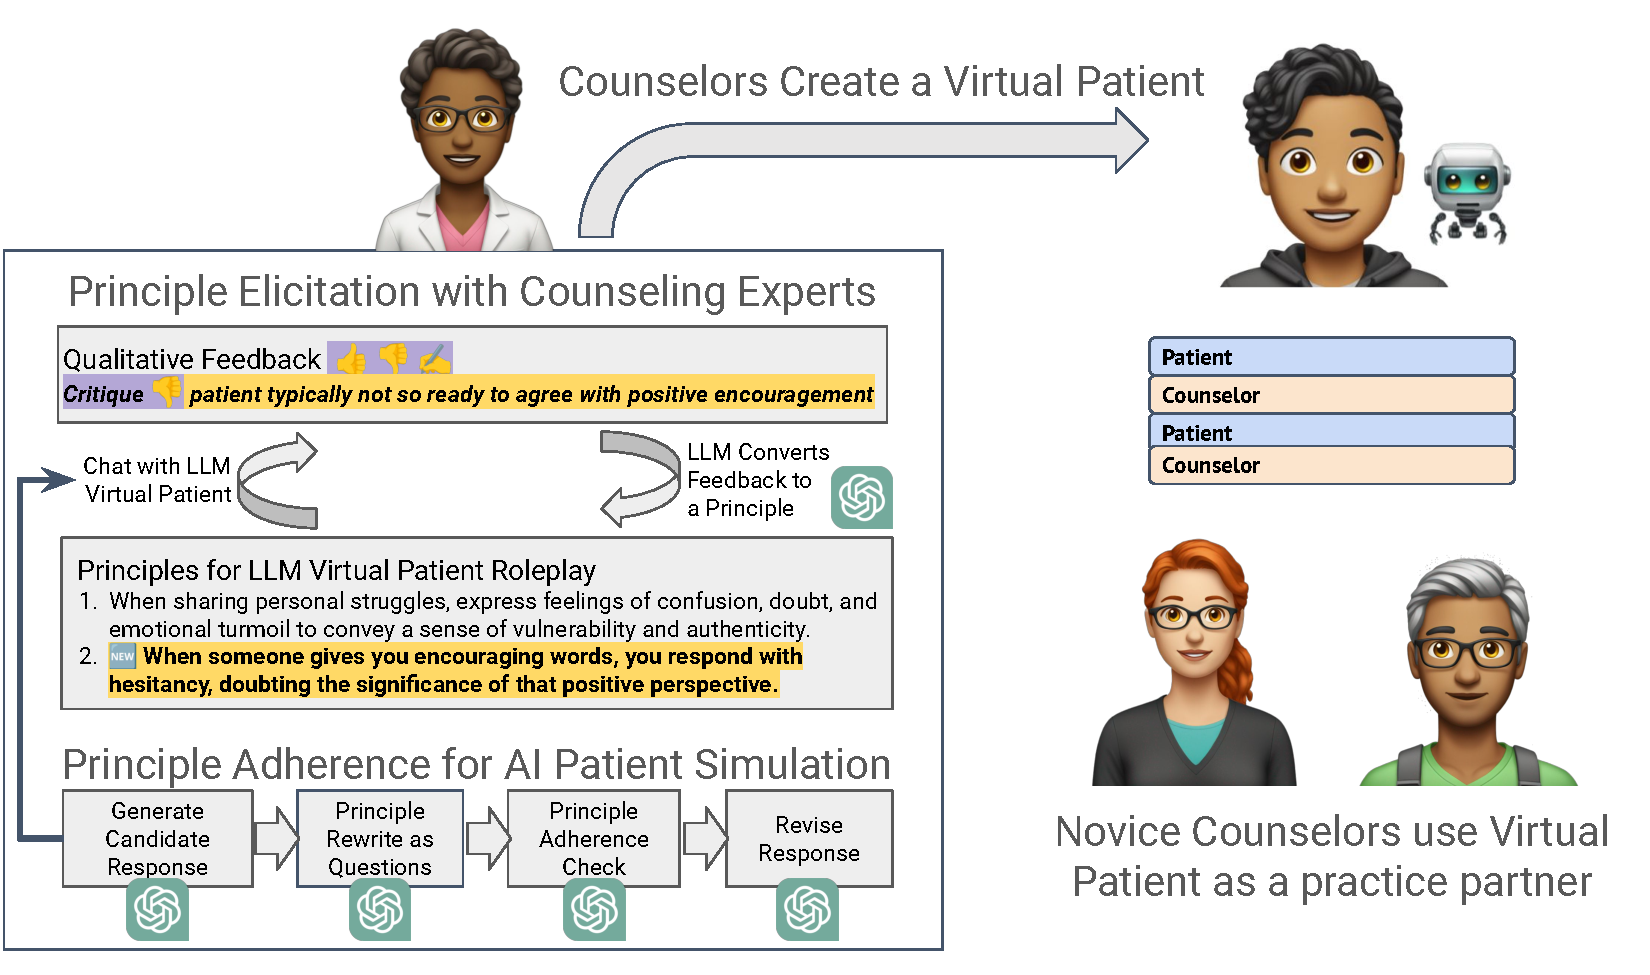
\includegraphics[width=\textwidth]{figures/rpdteaser.pdf}
    \caption{Roleplay-doh empowers a counseling expert to create a customized virtual patient intended for other novice counselors to use as a practice partner. During a chat, a counselor provides qualitative feedback as a kudos, critique, or rewrite which is converted by an LLM into a principle that is added to the constitution that governs the virtual patient roleplay, known as the \textbf{principle elicitation} process~\cite{petridis2023constitutionmaker}. When generating responses, the virtual patient self-critiques and revises its response for reliable \textbf{principle adherence}.}
    \label{fig:rpdteaser}
\end{figure*}


Collecting human feedback from counseling experts is therefore crucial for making authentic virtual patients.  However, standard approaches for collecting human preference data for aligning AI models~\cite{christiano2017deep, rafailov2024direct} are much too inefficient in terms of annotator-time and the iteration-time for testing a new model. 
Promisingly,~\citet{chen2023llmempowered} conduct qualitative feedback sessions with psychotherapy experts to understand how to better prompt the behaviors of LLMs to simulate a depressive patient. However, these co-design sessions are inefficient as it requires the researcher or system designer to convert a therapist's feedback of the virtual patient into a well-worded prompt, requiring multiple sessions before arriving at a authentic \diyi{instead of "authentic", should we call it "realistic"?}  simulation.
% While a more rapid approach could be prompting for desired simulation behaviors, domain-experts, who often fall into the category of non-technical users, struggle to prompt for simulation of desired personas~\cite{whyjohnnycantprompt}. 
In our work, \textbf{we consider how mental health experts can be empowered to construct their own virtual patient chatbot and shape its behaviors to more authentic in a single co-design session} \diyi{i don't know whether we should emphasize "single" (as opposed to multiple) co-design session here, nor the 30-min. i found these to be too specific details, rather than general scientific principles as a contribution statement.. }, enabling more rapid prototyping of authentic, AI roleplay partners for therapist training 
% \ananjan{Explicitly mentioning that it is a tool for codesign would probably help with the framing. Also mentioning that nothing similar exists} \diyi{it would be great to point out why this "constructor of virtual patient" idea is new compared to prior work; and what technical challenges exist (why it is hard). }  \emma{Can add in DPO / RLHF comparison.} 
\ryan{I could further show novelty of "active feedback loop" as opposed to more passive incorporation of expert feedback.}

Towards this goal, we introduce a novel human-AI collaboration pipeline for 
% developed an initial version of a tool 
counseling experts to construct LLM-prompted simulated patients within a 30 minute co-design session. Since therapists and experts may not know how to prompt for simulation of desired personas or behaviors~\cite{whyjohnnycantprompt}, our tool adopts a recent paradigm for user-driven chatbot design~\cite{petridis2023constitutionmaker} that allows users to rapidly prototype constitutional AI principles~\cite{bai2022constitutional} by simply providing natural language feedback on chatbot responses. \ryan{Flesh our the argument of our approach: (1) Experts have a lot of domain expertise for detecting good vs bad behaviors. (2) They are better at doing this than prompt engineering (CITE Samfirescu-Pereira paper); (3) Principle elicitation is a natural way to identify and articulate actionable principles that counselors believe are important} Via formative evaluations of the tool, we show the feasibility of eliciting counselor's qualitative feedback about authentic behaviors (e.g., disclosing too much at once;  being too articulate; needing to show more hesitancy) and converting them into principles that the LLM roleplay simulation should follow. However, results from additional tests revealed that a GPT-4 powered implementation of the method failed 20\% of the time to generate satisfying responses that adhere to the expert-written principles and stay consistent with the patient backstory and conversation history. \diyi{since this is a transition to your method, we can be brief here and briefly mention GPT-4 doesn't work if we just prompt it. }

% Unsatisfactory responses were due to LLMs not adhering to multiple criteria at once, misapplying principles that are only relevant for certain situations, and making responses that were unnatural for the dialogue context. \cheng{would it serve us better if we do not use the terms ``principles'' and ``principles'' interchangeably?} \ananjan{Probably too much detail for the introduction. Could just mention that we identify ways in which GPT-4 fails and design patches for them.}




Informed by our formative testing, we present \textbf{Roleplay-doh}, a co-design tool that enables counseling experts to effectively shape the behaviors an LLM-powered virtual patient through constitutional principles with additional checks to ensure principle following; see Figure~\ref{fig:rpdteaser}. \ryan{How does this contrast with the past paragraph? V2 of Roleplaydoh feels repetitive} With Roleplay-doh, counselors can construct a virtual help-seeker bot by (1) writing a roleplay scenario that describes a challenging past case; and (2) shaping the help-seeker bot's dialogue behaviors via natural language feedback that is converted into a set of well-defined principles. Roleplaydoh is a case of an LLM-powered system that empowers mental-health counseling experts to contribute directly to the advancement of LLM-powered dialogue-simulation training technologies--by providing them the tools to construct authentic virtual patients that aim to mirror challenging cases coming from their real-world therapy and counseling experience.   

To ensure that the dialogue-simulation adheres to the principles defined by counseling-experts, we develop a module for \textbf{principle-adherance} within the dialogue-simulation pipeline which \textit{critiques} a candidate response for its adherence to the principles and \textit{revises} the response according to the self-critique. While sharing similarities with general methods for self-refining an LLM's outputs~\cite{madaan2023selfrefine}, our \textit{principle-adherance} LLM program is specifically designed to (1) assess which user-defined principles and implicit criteria are relevant in the dialogue context and (2) decompose multipart and conditional principles into a set of yes/no principles that are easier to judge; see Figure~\ref{fig:agent-critique-improve}. These two key ideas for generating implicit principles and decomposing multifaceted principles into easier-to-evaluate dimensions bear a resemblance to the recent Branch-Solve-Merge~\cite{saha2023branchsolvemerge} LLM program for multi-faceted language generation and evaluation tasks. However, our approach is substantially more efficient than Branch-Solve-Merge in terms of LLM API calls, and results in large performance gains in our setting of simulating conversations between counselors and help-seekers.


% \ananjan{our task requires more abstract thinking than the tasks in BSM, potential point of difference. Our approach also makes a reduced number of LLM calls as compared to BSM} Roleplay-doh employs such ideas for principles evaluation as part of a self-critique-revise method to address challenges of LLM adhering to constitutional principles for faithful and realistic LLM simulations. \ananjan{repetition}

\if 0
% Alternative, original
Roleplay-doh's technical contribution is an LLM program for self-critique and revision that is capable of (1) assessing which explicit principles and implicit conventions are relevant to the dialogue context, (2) decomposing multipart and conditional principles into a set of yes/no principles and (3) answering these principles using chain-of-thought to guide the generation of a revised response; see Figure~\ref{fig:agent-critique-improve}. The generation of implicit principles and decomposing principles into easier-to-evaluate dimensions bears resemblance to the recent Branch-Solve-Merge~\cite{saha2023branchsolvemerge} LLM program for multi-faceted evaluation tasks. In this paper, we adapt these ideas as part of Roleplay-doh's self-critique method to address the challenges of LLM adhering to a set of principles for making simulations more faithful and realistic. 
\fi 

% To address the problems raised in this formative study, we collect over 100 test cases to benchmark methods for principle following in LLM roleplay simulations. We develop an LLM program for self-critique and improvement is capable of (1) assessing the set of explicit principles and unspoken conventions that are relevant to the dialogue context; (2) decomposing multipart and conditional principles into a set of yes/no principles; and (3) answering these principles in a chain-of-thought manner. The generation of implicit principles and decomposing principles into easier to evaluate dimensions bears resemblance to the recent Branch-Solve-Merge~\cite{saha2023branchsolvemerge} LLM program for multi-faceted language generation and evaluation tasks. This work employs such ideas used for critera evaluation as part of a self-critique method to address challenge of LLM roleplay simulations adhering to a set of principles.  
\ryan{When introducing eval methods, can emphasize more argument for why this kind eval is needed for human-LLM interaction}
We extensively evaluate Roleplay-doh from three perspectives. First, in a technical methods evaluation, we find that our full self-critique-improve module generates responses that are equally or more satisfying in terms of principle adherence, and reducing issues of awkward and inconsistent responses. Second, we conduct a within-subjects study (N=17) where counselors created virtual helpseeker bots with a \textit{Scenario-Only} method vs. Roleplay-doh's \textit{Scenario+ExpertPrinciples} method. Our results show that within a 30 minute co-design session, counselors can easily and effectively use the tool to create virtual helpseeker chatbots that are more authentic, exhibit behaviors that better recreate the challenging aspects of a case, are more ready and highly recommended as a practice partner---as judged from the perspective of creators and third-party counselors. Third, our analysis of the 85 principles elicted from counseling-experts highlights that while there many commonly-agreed upon principles (e.g., less articulate and willing to disclose, displaying emotional depth rather than stating emotion words, and expressing uncertainty in suggested coping strategies), more unique principles are also neccessary to faithfully simulate a diverse set of help-seekers, thus emphasizing the need for tools like Roleplaydoh to customize LLM-powered human simulations.

\diyi{this reads much better! one way to think about shortening the intro is to focus on our key contributions. Here are my perceived contributions: (1) using co-design to enable counselors to construct their own virtual patients; (2) use the insights from co-design to build roleplay-doh, which has the principle-adherence critique module (new); (3) such system works well (with brief description). More concretely, we are a bit slow to get to the key point, so it might be nice to merge the first three paragraphs in Intro to be one or two paragraphs, and use the next three paragraphs to illustrate the three contributions here. }


\section{Introduction - April 10th Outline}
\if 0
\begin{itemize}
\item     Realistic practice is key for novice counselors to learn how to apply active listening and clinical skills to support help-seekers.
\item     Standardized patients--human actors whom can authentically play the role of a patient scenario--have been a cornerstone in a clinical education. However, their cost and availability makes this practice-method impractical for the many novice counselors in-training.
\item   To meet this need, researchers have explored the potential of creating virtual patient's, that can roleplay as convincing AI dialogue partners for more  accessible practice.
\item   Historically, developing virtual helpseekers required training on counseling-datasets to behavioral clone multiple personas, but also suffered from the scarcity of publicly-available data due to data-privacy concerns. With powerful LLMs, an increasingly appealing method is prompting the LLM to roleplay a helpseeker persona and simulate the dialogue directly.
\item   However, directly prompting LLMs can create simulations that fail to exhibit authentic behaviors when judged by real therapists and counselors, as recent papers have found and which we also confirm in our studies with experienced-counselors.
\item Collecting human feedback from counseling experts is thus crucial for making authentic virtual patient's.  However, standard approaches for collecting human preference feedback for aligning LLMs (RLHF/DPO) are much too inefficient in terms of annotator-time and the iteration-time for testing a new model.
\item While a more rapid approach could be prompting for desired simulation behaviors, domain-experts, who often fall into the category of non-technical users, struggle to prompt for simulation of desired personas. 
\item In our work, we show that it's possible to use counselor's qualitative feedback (e.g., when self-disclosure is too much;  how the style of speech or vocabulary should be changed;  situations where real patients show more resistance) rapidly prototype [constitutions, or sets of principles that govern agent behavior, for more] authentic LLM-simulated patients within a 30 minute co-design session.
\item 
\end{itemize}
\fi
\section{Introduction - April 8th Edits}


Large Language Models (LLMs) that can roleplay as different characters~\citep{park2022social, park2023generative} could be used as convincing AI dialogue partners for training social skills, such as being used as simulated-students for TA training~\citep{markel_opferman_landay_piech_2023} or a simulated-patients for psychotherapy training~\citep{chen2023llmempowered}. 
AI roleplay partners have the potential to enable virtual practice environments that help make social skill training more inviting compared to having to acquire such skills on the job, and accessible for learners who do not have dedicated human partners to readily train with~\citep{yang2024social}. Faithfulness and realism are crucial for making these simulated roleplays more immersive and useful, and ensuring that the skills learned may better transfer to real-world situations~\cite{alinier2022simulation}. \diyi{instead of a broader opening, it might be nice to just emphasize the need of virtual patients in empowering novice counselors, as the current 1st paragraph is a bit broad.}

%  
\diyi{standardized patients concept exist for a long time, even before LLMs. we should justify for why LLM based virtual patient is needed. Then among existing efforts to build LLM based virtual patients, why they are not enough? Then it would motivate our work of co-designing + principles ...}
Within the area of mental health, language models have been used to simulate clients in counseling conversations~\citep{tanana2019development}, people seeking support in times of crisis~\citep{demasi-etal-2020-multi}, and depressive patients~\citep{chen2023llmempowered}. Prior work has created simulations of diverse help-seekers from two perspectives. The first approach uses behavioral cloning to create convincing simulations by mimicking a dataset of mental health conversations, with an emphasis on modeling multiple personas in the data~\citep{tanana2019development, chiu2024computational}. However, publicly available mental health datasets are scarce, making this less practical in practice. The second approach directly prompts LLMs to roleplay different patients with varying symptoms or issues. Direct prompting provides the flexibility to easily customize the patient simulation, but requires specific prompts about the conversation behaviors to make them faithful to the behaviors of real patients in mental health conversations. Promisingly,~\citet{chen2023llmempowered} co-design the prompts for faithful conversation behaviors of a depressive patient \textit{collaboratively with psychotherapy experts}. However, their co-design method is inefficient as it requires the researcher or system designer to convert a therapist's feedback on the patient bot into a well-worded prompt, requiring multiple co-design sessions before arriving at a final prompt. Therefore, \textbf{our work asks whether mental health experts can be empowered to interactively shape the conversation behaviors of LLM-prompted patient simulations}, enabling more rapid co-design of faithful and authentic roleplay partners for therapist skill training. 
\ananjan{Explicitly mentioning that it is a tool for codesign would probably help with the framing. Also mentioning that nothing similar exists} \diyi{it would be great to point out why this "constructor of virtual patient" idea is new compared to prior work; and what technical challenges exist (why it is hard). } \ryan{This second paragraph should better resolve these comments}
\emma{Can add in DPO / RLHF comparison.}

Towards this goal, we developed an initial version of a tool for counseling experts to construct LLM-prompted simulated patients. Since therapists and experts may not know how to prompt for simulation of desired personas or behaviors~\cite{whyjohnnycantprompt}, our tool adopts a recent paradigm for user-driven chatbot design~\cite{petridis2023constitutionmaker} that allows users to rapidly prototype constitutional rules~\cite{bai2022constitutional} by simply providing natural language feedback on chatbot responses. Results from our formative evaluations of the tool showed that while this paradigm helped counseling experts identify and articulate principles that realistic simulations should follow, a GPT-4 powered implementation of the method failed 20\% of the time to generate satisfying responses that adhere to the expert-written principles and stay consistent with the patient backstory and conversation history. 

% Unsatisfactory responses were due to LLMs not adhering to multiple criteria at once, misapplying principles that are only relevant for certain situations, and making responses that were unnatural for the dialogue context. \cheng{would it serve us better if we do not use the terms ``principles'' and ``principles'' interchangeably?} \ananjan{Probably too much detail for the introduction. Could just mention that we identify ways in which GPT-4 fails and design patches for them.}

\begin{figure}[t]
    \centering
    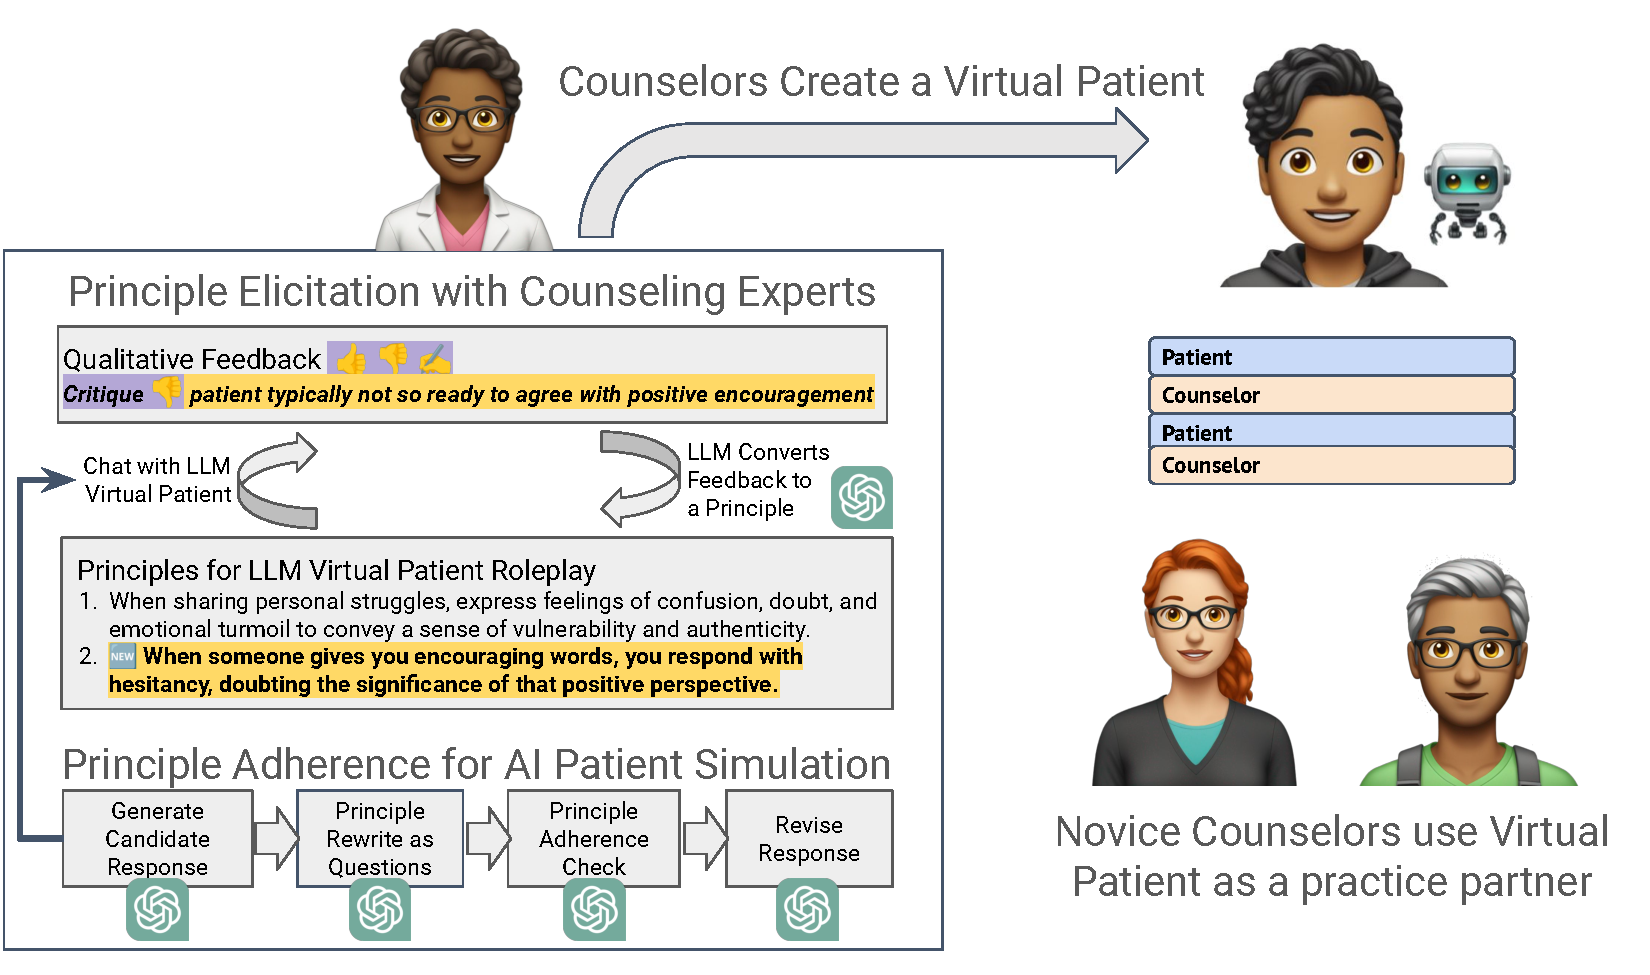
\includegraphics[width=\columnwidth]{figures/rpdteaser.jpg}
    \caption{Roleplay-doh supports a domain expert in shaping LLM simulations to be faithful and realistic for roleplay. Natural language feedback is elicited while a domain-expert chats which is converted into a constitution consisting of principles that the LLM roleplay should follow. Roleplay-doh also uses LLMs to self-critique and revise its responses that better adhere to the expert-defined principles.\ryan{Handsketched teaser, needs a higher-fidelity with examples}}
    \label{fig:rpdteaser}
\end{figure}


Informed by our formative testing, we present \textbf{Roleplay-doh}, a co-design tool that enables counseling experts to effectively shape the behaviors of LLM simulators through constitutional principles with additional checks to ensure principle following; see Figure~\ref{fig:rpdteaser}. With Roleplay-doh, counselors can construct a virtual help-seeker bot by (1) writing a roleplay scenario that describes a challenging past case; and (2) shaping the help-seeker bot's dialogue behaviors via natural language feedback that is converted into a set of well-defined principles. Roleplaydoh is a case of an LLM-powered system that empowers mental-health counseling experts to contribute directly to the advancement of LLM-powered dialogue-simulation training technologies--by providing them the tools to construct authentic virtual patients that aim to mirror challenging cases coming from their real-world therapy and counseling experience.   

To ensure that the dialogue-simulation adheres to the principles defined by counseling-experts, we develop a module for \textbf{principle-adherance} within the dialogue-simulation pipeline which \textit{critiques} a candidate response for its adherence to the principles and \textit{revises} the response according to the self-critique. While sharing similarities with general methods for self-refining an LLM's outputs~\cite{madaan2023selfrefine}, our \textit{principle-adherance} LLM program is specifically designed to (1) assess which user-defined principles and implicit criteria are relevant in the dialogue context and (2) decompose multipart and conditional principles into a set of yes/no principles that are easier to judge; see Figure~\ref{fig:agent-critique-improve}. These two key ideas for generating implicit principles and decomposing multifaceted principles into easier-to-evaluate dimensions bear a resemblance to the recent Branch-Solve-Merge~\cite{saha2023branchsolvemerge} LLM program for multi-faceted language generation and evaluation tasks. However, our approach is substantially more efficient than Branch-Solve-Merge in terms of LLM API calls, and results in large performance gains in our setting of simulating conversations between peer counselors and help-seekers.


% \ananjan{our task requires more abstract thinking than the tasks in BSM, potential point of difference. Our approach also makes a reduced number of LLM calls as compared to BSM} Roleplay-doh employs such ideas for principles evaluation as part of a self-critique-revise method to address challenges of LLM adhering to constitutional principles for faithful and realistic LLM simulations. \ananjan{repetition}

\if 0
% Alternative, original
Roleplay-doh's technical contribution is an LLM program for self-critique and revision that is capable of (1) assessing which explicit principles and implicit conventions are relevant to the dialogue context, (2) decomposing multipart and conditional principles into a set of yes/no principles and (3) answering these principles using chain-of-thought to guide the generation of a revised response; see Figure~\ref{fig:agent-critique-improve}. The generation of implicit principles and decomposing principles into easier-to-evaluate dimensions bears resemblance to the recent Branch-Solve-Merge~\cite{saha2023branchsolvemerge} LLM program for multi-faceted evaluation tasks. In this paper, we adapt these ideas as part of Roleplay-doh's self-critique method to address the challenges of LLM adhering to a set of principles for making simulations more faithful and realistic. 
\fi 

% To address the problems raised in this formative study, we collect over 100 test cases to benchmark methods for principle following in LLM roleplay simulations. We develop an LLM program for self-critique and improvement is capable of (1) assessing the set of explicit principles and unspoken conventions that are relevant to the dialogue context; (2) decomposing multipart and conditional principles into a set of yes/no principles; and (3) answering these principles in a chain-of-thought manner. The generation of implicit principles and decomposing principles into easier to evaluate dimensions bears resemblance to the recent Branch-Solve-Merge~\cite{saha2023branchsolvemerge} LLM program for multi-faceted language generation and evaluation tasks. This work employs such ideas used for critera evaluation as part of a self-critique method to address challenge of LLM roleplay simulations adhering to a set of principles.  

In a technical methods evaluation, we find that Roleplay-doh's self-critique-revise program is preferred in 65\% of cases compared to the baseline of directly prompting GPT-4 to follow the principles. \ananjan{This number is weak, need a better way of stating this. This is also inaccurate, it has a win rate of 65\% over \textit{all} ablations} We perform ablations to verify the utility of each component of our proposed self-critique-revise approach. Additionally, we conduct a within-subjects study (N=17) where mental health experts created simulation partners with a \textit{Scenario-Only} method vs. our \textit{Scenario+ExpertPrinciples} method using Roleplaydoh to add principles to shape behaviors. Creator's answers to our questionnaire indicate that Roleplaydoh empowers them to define principles that effectively shape roleplays, and that their expert principles make the simulations more authentic ($d=.66$), more faithful recreations of the past case ($d=.59$) and its challenging aspects ($d=.76$), and more ready to be used as simulation partners ($d=.93$). We also conduct in-depth analyses of the scenarios and principles that creators made, and share implications for using expert-defined principles as general ways to customize patients and clients for simulated mental health dialogues.  
% We recruitied participants that were familiar with online peer counseling conversations and thus were capable of comparing the LLM-simulation partners to their real-world experiences. 
We complement the creator's perspective with external evaluations of the simulated-dialogues collected during the creator study. We find a similar sized effect when \textit{other counselors} offer a third-party judgement of the simulated helpseekers with/without expert principles. Via an automatic analysis of the conversations, we find that help-seeker response are less verbose and therapist's use later-converation strategies (e.g., problem-solving and planning) 1.65 turns later in the dialogues, which highlights the benefits for realistic practice of therapy skills.

In summary, this paper makes the following contributions:
\begin{itemize}
    \item The paper presents Roleplay-doh, a tool enabling domain experts to create realistic LLM-agent simulations for training.
    \item A formative study with experts in peer counseling validated the tool's efficacy in converting expert feedback into guiding principles, but also highlighted challenges in instructing language models (like GPT-3.5 and GPT-4) to adhere to complex sets of principles.
    \item In response, we develop a novel module within RolePlay-doh to ensure better principle adherence, through a breaking down of explicit complex principles into smaller principles, generating additional context-relevant principles, and employing a self-critique and improvement approach to refine responses. 
    \item Roleplay-doh's self-critique-revise program can achieve greater principle adherance and is ranked the most satisfactory compared to directly prompting GPT4 as well as several other similar baselines. Our final evaluations with peer counselors further shows that our tool enables experts to shape LLM simulators to be more realistic from their first-person experience and based on third-person jugements.
\end{itemize}

% Taken together, these findings highlight the importance of tools and methods that empower domain experts to articulate their principles for realism and effectively shape LLM roleplay behaviors around them; we believe this can inform the design of future expert-defined LLM simulators for social skill training. \ananjan{this feels a bit disjointed. Could wrap up by reiterating that our tool is effective, quantitatively better than vanilla GPT-4 and opens up directions for future research in this direction as well as application to more domains.}

\diyi{the intro is great! i might highlight more about a few dimensions: (1) we can use "principle adherence" as the keyword to denote our method; (2) we should frame the work as "LLM-empowered system to empower therapists, and touch more on the human-AI interaction system. The potential submission track should be "human-centered nlp" or "nlp applications" to avoid critical R2; (3) emphasize more about "utility" evaluation and frame this as a new way to improve evaluation in the age of LLMs for better human-AI interaction system.}
\ananjan{should call out the distinctions between our work and previous. e.g., Branch solve merge does not evaluate in the domain of roleplay. Also agree on point (3) above, the introduction does not really emphasize on our comprehensive user evaluations. Maybe we could showcase a few cases where quantitative automated evaluation metrics fail?}
\cheng{It sounds like the introduction is trying to claim that roleplay-doh is a system applicable to domains other than mental health counseling. If so, would it be better to clarify at some point that experiments were conducted with participants and data from the peer-to-peer counseling domain?}
\emma{Looks great! I also agree with the others' comments. I would further emphasize the key limitations of other approaches (even if there's one dataset, there may not be for a new particular type of therapy or domain), why this is non-trivial to do well, that these ideas could be used for other types of simulate-person-X settings; that this is a a highly efficient way (we think) to get useful input from experts in order to create customizable simulated humans (aka are the principles similar? different?).}

\section{Introduction - April 8th copy before edits}
\section{Introduction}
There has been growing interest in using LLMs for simulating human behavior ~\cite{park2023generative, park2022social, zhou2023sotopia} to expedite tasks such as data annotation and subjective model evaluation. One such promising application is the use of chatbots and LLMs to simulate role-playing partners for social skill training~\cite{othlinghaus2020seriousroleplaying, markel_opferman_landay_piech_2023, chen2023llmempowered}). These models are often cheaper, more scalable, and less high-stakes \ananjan{this sounds odd} when compared to practicing with a human. Faithfulness and realism are crucial for making these simulated roleplays more immersive and useful, and ensuring that the skills learned may better transfer to real-world situations~\cite{alinier2022simulation}.  Additionally, as experienced peer counselors have faced challenging moments from their personal experience, such scenarios are valuable to turn into simulated scenarios for novice counselors to practice with. Thus, a key goal in this work is empowering peer counseling experts to shape LLM-simulated roleplays to be a faithful and realistic recreation of challenging real-world cases. 
% Faithfulness and realism are crucial for making these simulated interactions more immersive and useful, and ensuring that the skills learned may better transfer to real-world situations~\cite{alinier2022simulation, cheng-etal-2023-compost}.


Despite many recent work showing how LLMs can be prompted to take on different personas~\cite{park2023generative}--and interfaces for customizing those personas along predefined character traits (e.g., CharacterAI)--it remains unclear what domain experts, like a peer counselor, would need to customize an LLM persona to recreate a challenging patient case that they have faced during their personal experiences. A core limitation in customization approaches is that they either provide preset dimensions for customization that may not match the granularity for personalizing the simulation to a specific scenario, or they require the user to perform careful prompting to elicit desired responses. As validated by recent studies ~\cite{whyjohnnycantprompt}, domain experts, who often fall into the category of non-technical users, struggle to prompt for simulation of desired personas.  Enabling experts to develop LLM-powered roleplay partners without technical supervision would allow for more rapid development of useful simulations, while simultaneously providing better feedback on faithfulness and realism from expert perspectives for iterative improvement and co-design. This paper develops a novel approach to achieve this goal in the context of simulating roleplay partners for peer counseling training. \ananjan{Explicitly mentioning that it is a tool for codesign would probably help with the framing. Also mentioning that nothing similar exists} \diyi{it would be great to point out why this "constructor of virtual patient" idea is new compared to prior work; and what technical challenges exist (why it is hard). }

We first evaluate an existing paradigm for user-driven chatbot design~\cite{petridis2023constitutionmaker} that allows users to iteratively provide natural language feedback on chatbot responses, which are then automatically converted into {\em constitution principles} that an LLM is instructed to follow. Results from our formative evaluations showed that while this paradigm helped counseling experts identify and articulate principles that realistic simulations should follow, a GPT-4 powered implementation of the method failed 20\% of the time to generate satisfying responses that adhere to the expert-written principles and stay consistent with the patient backstory and conversation history. 

% Unsatisfactory responses were due to LLMs not adhering to multiple criteria at once, misapplying principles that are only relevant for certain situations, and making responses that were unnatural for the dialogue context. \cheng{would it serve us better if we do not use the terms ``principles'' and ``principles'' interchangeably?} \ananjan{Probably too much detail for the introduction. Could just mention that we identify ways in which GPT-4 fails and design patches for them.}

\begin{figure}[t]
    \centering
    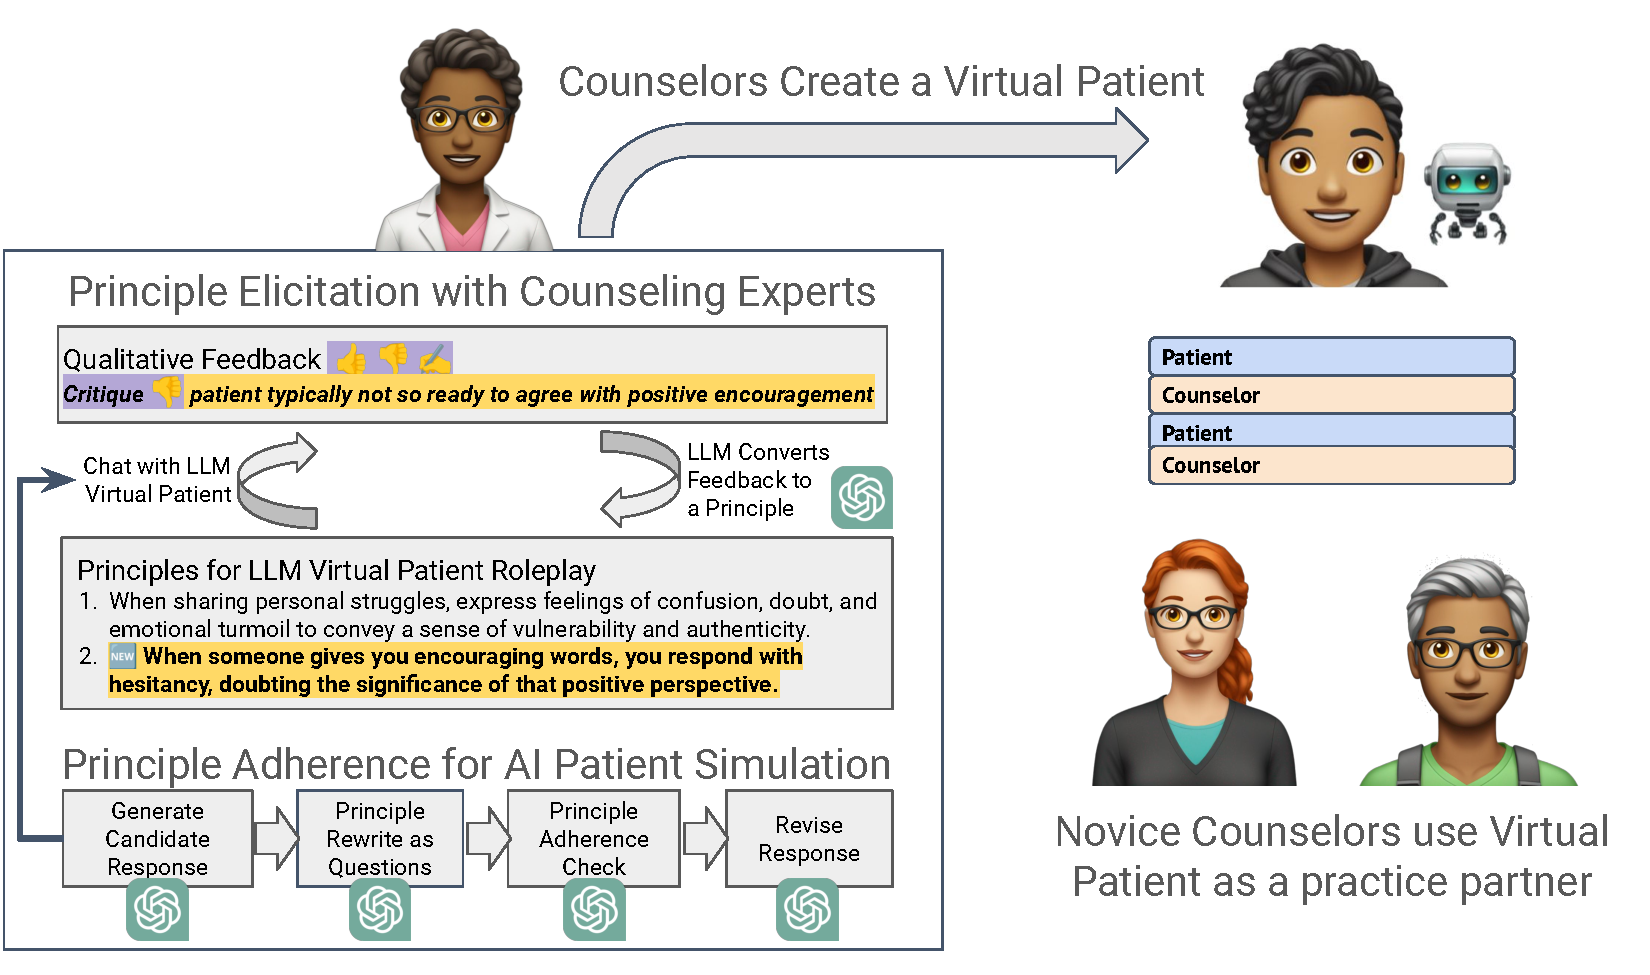
\includegraphics[width=\columnwidth]{figures/rpdteaser.jpg}
    \caption{Roleplay-doh supports a domain expert in shaping LLM simulations to be faithful and realistic for roleplay. Natural language feedback is elicited while a domain-expert chats which is converted into a constitution consisting of principles that the LLM roleplay should follow. Roleplay-doh also uses LLMs to self-critique and revise its responses that better adhere to the expert-defined principles.\ryan{Handsketched teaser, needs a higher-fidelity with examples}}
    \label{fig:rpdteaser}
\end{figure}

To address this problem, we propose Roleplay-doh, a tool that enables counseling experts to effectively shape the behaviors of LLM simulators through constitutional principles with additional checks to ensure principle following; see Figure~\ref{fig:rpdteaser}. With Roleplay-doh, counselors can construct a virtual help-seeker bot by (1) writing a roleplay scenario that describes a challenging past case; and (2) shaping the help-seeker bot's dialogue behaviors via natural language feedback that is converted into a set of well-defined principles. To ensure that the LLM dialogue simulator adheres to the counseling expert's principles, Roleplay-doh uses LLMs to generate a candidate response, critique its adherence to user principles, and revise the response according to the self-critique. 

The self-critique-revise LLM program is specifically designed to (1) assess which user-defined principles and implicit criteria are relevant in the dialogue context; and (2) decompose multipart and conditional principles into a set of yes/no principles that are easier to judge; see Figure~\ref{fig:agent-critique-improve}. These two key ideas for generating implicit principles and decomposing multifaceted principles into easier-to-evaluate dimensions bear a resemblance to the recent Branch-Solve-Merge~\cite{saha2023branchsolvemerge} LLM program for multi-faceted language generation and evaluation tasks. However, our approach is substantially more efficient than Branch-Solve-Merge in terms of LLM API calls, and results in large performance gains in our setting of simulating conversations between peer counselors and help-seekers.

% \ananjan{our task requires more abstract thinking than the tasks in BSM, potential point of difference. Our approach also makes a reduced number of LLM calls as compared to BSM} Roleplay-doh employs such ideas for principles evaluation as part of a self-critique-revise method to address challenges of LLM adhering to constitutional principles for faithful and realistic LLM simulations. \ananjan{repetition}

\if 0
% Alternative, original
Roleplay-doh's technical contribution is an LLM program for self-critique and revision that is capable of (1) assessing which explicit principles and implicit conventions are relevant to the dialogue context, (2) decomposing multipart and conditional principles into a set of yes/no principles and (3) answering these principles using chain-of-thought to guide the generation of a revised response; see Figure~\ref{fig:agent-critique-improve}. The generation of implicit principles and decomposing principles into easier-to-evaluate dimensions bears resemblance to the recent Branch-Solve-Merge~\cite{saha2023branchsolvemerge} LLM program for multi-faceted evaluation tasks. In this paper, we adapt these ideas as part of Roleplay-doh's self-critique method to address the challenges of LLM adhering to a set of principles for making simulations more faithful and realistic. 
\fi 

% To address the problems raised in this formative study, we collect over 100 test cases to benchmark methods for principle following in LLM roleplay simulations. We develop an LLM program for self-critique and improvement is capable of (1) assessing the set of explicit principles and unspoken conventions that are relevant to the dialogue context; (2) decomposing multipart and conditional principles into a set of yes/no principles; and (3) answering these principles in a chain-of-thought manner. The generation of implicit principles and decomposing principles into easier to evaluate dimensions bears resemblance to the recent Branch-Solve-Merge~\cite{saha2023branchsolvemerge} LLM program for multi-faceted language generation and evaluation tasks. This work employs such ideas used for critera evaluation as part of a self-critique method to address challenge of LLM roleplay simulations adhering to a set of principles.  

In a technical methods evaluation, we find that Roleplay-doh's self-critique-revise program is preferred in 65\% of cases compared to the baseline of directly prompting GPT-4 to follow the principles. \ananjan{This number is weak, need a better way of stating this. This is also inaccurate, it has a win rate of 65\% over \textit{all} ablations} We perform ablations to verify the utility of each component of our proposed self-critique-revise approach. We also conduct a final user evaluation study investigating whether LLM-simulation partners using expert-shaped principles are perceived as being more realistic and relevant for training of peer counselors than a baseline GPT-4 model that is instructed to roleplay a persona without the guiding principles.
% We recruitied participants that were familiar with online peer counseling conversations and thus were capable of comparing the LLM-simulation partners to their real-world experiences. 
An external set of peer counselor "judges" (N=20) interacted with the LLM-simulation partners---which were either a baseline roleplay prompt or the ones made with expert-defined principles.
Our results show that expert-shaped LLM-simulation partners are perceived as playing the role more authentically and realistically, are more ready to be used as a simulation partner, support greater immersion in the conversation, and can help listeners encounter more challenging scenarios which are useful for practice.\ryan{Note: These are expected findings, this end-user evaluation study has not been completed.} \ananjan{would be helpful to put a few percentages here once the studies are done! could be put in abstract as well.}



In summary, this paper makes the following contributions:
\begin{itemize}
    \item The paper presents Roleplay-doh, a tool enabling domain experts to create realistic LLM-agent simulations for training.
    \item A formative study with experts in peer counseling validated the tool's efficacy in converting expert feedback into guiding principles, but also highlighted challenges in instructing language models (like GPT-3.5 and GPT-4) to adhere to complex sets of principles.
    \item In response, we develop a novel module within RolePlay-doh to ensure better principle adherence, through a breaking down of explicit complex principles into smaller principles, generating additional context-relevant principles, and employing a self-critique and improvement approach to refine responses. 
    \item Roleplay-doh's self-critique-revise program can achieve greater principle adherance and is ranked the most satisfactory compared to directly prompting GPT4 as well as several other similar baselines. Our final evaluations with peer counselors further shows that our tool enables experts to shape LLM simulators to be more realistic from their first-person experience and based on third-person jugements.
\end{itemize}

% Taken together, these findings highlight the importance of tools and methods that empower domain experts to articulate their principles for realism and effectively shape LLM roleplay behaviors around them; we believe this can inform the design of future expert-defined LLM simulators for social skill training. \ananjan{this feels a bit disjointed. Could wrap up by reiterating that our tool is effective, quantitatively better than vanilla GPT-4 and opens up directions for future research in this direction as well as application to more domains.}

\diyi{the intro is great! i might highlight more about a few dimensions: (1) we can use "principle adherence" as the keyword to denote our method; (2) we should frame the work as "LLM-empowered system to empower therapists, and touch more on the human-AI interaction system. The potential submission track should be "human-centered nlp" or "nlp applications" to avoid critical R2; (3) emphasize more about "utility" evaluation and frame this as a new way to improve evaluation in the age of LLMs for better human-AI interaction system.}
\ananjan{should call out the distinctions between our work and previous. e.g., Branch solve merge does not evaluate in the domain of roleplay. Also agree on point (3) above, the introduction does not really emphasize on our comprehensive user evaluations. Maybe we could showcase a few cases where quantitative automated evaluation metrics fail?}
\cheng{It sounds like the introduction is trying to claim that roleplay-doh is a system applicable to domains other than mental health counseling. If so, would it be better to clarify at some point that experiments were conducted with participants and data from the peer-to-peer counseling domain?}



\section{Introduction}

% There's increasing interest in using LLMs for simulating human behavior ~\cite{park2023generative, park2022social, zhou2023sotopia}. One promising application is using LLMs to simulate persons with which users can practice and rehearse social interactions and communication scenarios (e.g., simulated students for TA training~\cite{markel_opferman_landay_piech_2023}; simulated patients for therapist training~\cite{chen2023llmempowered}) as they enable cheaper, scalable, and less high-stakes ways to practice without requiring another human. ~\cite{markel_opferman_landay_piech_2023, park2022social}. Faithfulness and realism is key to make these simulations impactful in critical settings~\cite{cheng-etal-2023-compost}. Despite many methods for simulating human personas~\cite{park2023generative} and products built on this idea (CharacterAI and OpenAI "GPTs"), studies show non technical users struggle to prompt for simulation (Why Johnny). Enabling experts to develop simulations on their own would allow more rapid development of simulations, while simultaneously providing better feedback on faithfulness and realism from expert perspectives. We try to do that in this work.

Chatbots powered by LLMs are being used as simulators of human behavior.  One important class of simulated agents are those that can engage in role-play activities. These can power practice and training technologies (e.g., training counselors for difficult mental health conversations~\cite{demasi-etal-2020-multi}, helping teaching assistants simulate interactions with students~\cite{markel_opferman_landay_piech_2023}, rehearsing conflict scenarios~\cite{shaikh2023rehearsal}).  In such application scenarios, it’s important for chatbot behaviors to capture diversity of personas encountered in real-world scenarios (for representative and challenging cases), and produce responses that are faithful to that realistic experience. In this paper, we are particulary interested in the application scenario of creating LLM-powered simulated help seekers, that can be used as practice partners for psychotherapy and peer counseling conversations~\cite{demszky2023using}. 

A core challenge to making realistic LLM simulations for conversational role play is ensuring a roleplay is authentic and faithful to realistic behaviors.  For example, if we are creating a simulated help seeker for a peer counseling platform, an LLM needs to exhibit the linguistic styles and behavioral tendencies of someone seeking help through an online platform.  While making such a realistic help seeker would be easier if this was trained on real-world data~\cite{demasi-etal-2020-multi}, data privacy considerations in sensitive domains like mental health and psychotherapy can limit access to real-world data a model can be fine-tuned on. Instead, a more common approach is to Prompt LLMs to simulate these conversations.
They avoid the issue of private data for such sensitive domains, prompting LLMs to take on a roleplay persona provides flexibility defining tailored background and character trait information~\cite{park2023generative, zhou2023sotopia}. While a character trait can be controlled via a persona, how do we ensure that the LLM agent acts realistically to that trait. For example, even if we create a persona of someone who is angry, how do we ensure the LLM roleplay conveys that anger through language in a way that might reminds a support seeker of a real-experience they have had?  We emphasize that despite lots of recent work on studying and evaluating LLMs roleplay abilities~\cite{zhou2023sotopia}, faithfulness to real-world conversations and behaviors is an understudied criteria that is important for user-facing interactions with an LLM-agent as practice partner to be authentic for for simulation-based training.

Such questions of faithfulness to the real-world call for involvement and feedback from experts who are familiar with conversations in a highly-specific domain. Prior research methods for engaging domain experts is as annotators (e.g., RLHF), or as user testers of a system in which they provide verbal feedback and system designers can iterate on the design -- in this case -- the prompts to the LLM to better align.  The feedback loop for this process is long and involved. Given LLMs highly configurable nature, there is a strong potential to remove a system designer from this loop, and enable experts such as a peer counselor to shape the LLM agent's behaviors themselves. In this work, we seek to develop tools and methods that enable domain-experts to construct an LLM-powered roleplay agent on their own that authentically represents real-world scenarios. 


To enable expert-constructed LLM practice partners, we built Roleplay-doh, tool for shaping the chatbot behaviors to be faithful to realistic scenarios; see Figure~\ref{fig:rpd}. We design it specifically to enable domain experts in mental health conversations to construct their own simulated support seekers and shape these behaviors. To support the interactive development of the roleplay agent's prompts, RolePlay-doh adopts the principle-elicitation techniques introduced in ConstitutionMaker~\cite{petridis2023constitutionmaker}, that allows users to provide natural-language {\em feedback} in terms of a kudos, critique, or rewrite on the LLM-agent's dialogue response which gets converted into well-structured and worded {\em principles} that are added to a {\em constitution} that the LLM agent is instructed to follow. We hypothesized that such an approach would empower domain experts in psychotherapy and peer counseling to construct and shape chatbot behaviors in real-time, eliminating the need for researchers or system designers to refine roleplay prompts after domain-experts provide feedback.


to address the categorical errors we observed when instructing LLM simulators to follow constitutional principles.   our agent program as shown in Figure~\ref{fig:agent-critique-improve} (1) produces a candidate response; (2a) formulates conditional and complex principles into a set of smaller yes/no criteria; (2b) uses an LLM to generate a set of general criteria that should be followed given a conversation context (e.g., when asked a question, answer it); (3) evaluates the candidate response on these criteria using a chain-of-thought approach; and  


As our first contribution, we conducted formative pilot sessions (N=6) with experts on an online peer counseling platform to inform our design iterations of Roleplay-doh. 
% Our goals were to understand (1) what principles are elicited from domain experts to guide more faithful real-world behaviors, and (2) what ways the tool could be improved to support domain experts in more effectively making and shaping these roleplay behaviors. 
We find that participants can easily and efficiently convert their feedback into principles with the principle elicitation approach used in RolePlay-doh. Nonetheless, we found that instruction-tuned LLMs like GPT-3.5 and GPT-4 could struggle to adhere to all the principles a domain-expert has written; this occured when there were (1) many principles to follow; (2) conditional principles that only apply during specific situations in the dialogue; and (3) complex principles composed of multiple criteria.  These challenges highlighted the limitations of simply instructing an LLM to follow such a set of principles, and the need for an improved backend LLM agent architecture that can ensure effective principle following during dialogue.

Thus, as our second contribution, our final design iteration of Roleplay-doh uses an agent architecture to produce dialogue responses that reliably follow the principles while remaining relevant to the dialogue context.  Inspired by the self-critique and branch-solve-merge~\cite{saha2023branchsolvemerge} LLM program patterns, our agent program as shown in Figure~\ref{fig:agent-critique-improve} (1) produces a candidate response; (2a) formulates conditional and complex principles into a set of smaller yes/no criteria; (2b) uses an LLM to generate a set of general criteria that should be followed given a conversation context (e.g., when asked a question, answer it); (3) evaluates the candidate response on these criteria using a chain-of-thought approach; and (4) produces a final revised response that better meets the explicit and implicit criteria. We evaluate the effectiveness of this self-critique-improve program architecture over (A) the baseline approach of a single call to GPT-4 to generate a dialogue response that follows the principles; (B) an ablation where principles are not written as criteria; and (C) an ablation which does not generate a set of implicit criteria for dialogue relevance.  We find that Roleplay-dohs LLM program architecture  produces responses that follow the principles and are relevant to the dialogue context than other approaches, while only adding an average of ~10 seconds more latency, which is acceptable in a simulation setting where partners are expected to take time to type their responses.\ryan{Note: These are expected findings, this comparison study has not been completed.}

Our final contribution is a user evaluation study investigating whether LLM-simulation partners using expert-shaped principles are perceived as being more realistic and relevant for training than a baseline GPT-4 model that is instructed to roleplay a persona (without the guiding principles).
% We recruitied participants that were familiar with online peer counseling conversations and thus were capable of comparing the LLM-simulation partners to their real-world experiences. 
An external set of peer counselor "judges" (N=20) interacted with the LLM-simulation partners---which were either a baseline model or the ones used expert-shaped principles defined by an initial set of expert peer counselors (N=6).
Our results show that expert-shaped LLM-simulation partners are perceved as playing the role more authentically and realistically, are more ready to be used as a simulation partner, supported greater immersion in the conversation, and can help listeners encounter more challenging scenarios which are useful for practice.\ryan{Note: These are expected findings, this end user evaluation study has not been completed}



\begin{figure*}[t]
    \centering
    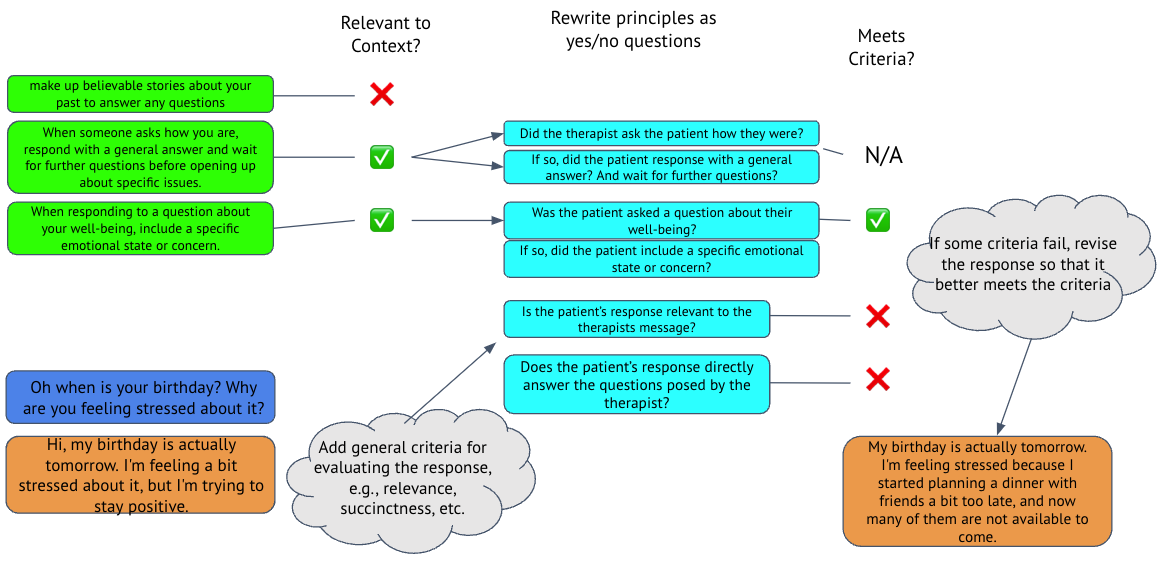
\includegraphics[width=\textwidth]{figures/agent-critique-improve-ex.png}
    \caption{LLM Program for more reliable constitution principle following}
    \label{fig:agent-critique-improve}
\end{figure*}

In summary, this paper makes the following contributions:
\begin{itemize}
    \item The paper presents RolePlay-doh, a tool enabling domain experts to create realistic LLM-agent simulations for training.
    \item The initial testing with experts in peer counseling revealed the tool's efficacy in converting expert feedback into guiding principles, but also highlighted challenges in instructing language models (like GPT-3.5 and GPT-4) to adhere to complex sets of principles.
    \item It introduces an improved chatbot architecture within RolePlay-doh for better principle adherence, through a breaking down explicit principles into smaller criteria, generating additional context-relevant criteria, and employing a self-critique and improvement approach to refine responses. The effectiveness of this architecture over tarditional models is demonstrated, offering responses that are more aligned with the set principles while maintaining relevance to the conversation context.
    \item Our user evaluations provide initial evidence that these expert-shaped chatbots offer more authentic and  effective training experiences in peer counseling scenarios.
\end{itemize}

Taken together, these findings highlighting the importance of tools/methods to empower domain experts to shape LLM roleplay behaviors and inform the design of future LLM-powered practice partners.

\section{Related Work}

% Social-science theory describing how utility is conditional on the immersiveness/realism?
\if 0
Faithfulness and realism are key to make these simulated interactions more immersive and useful so that the skills learned may transfer to real-world situations~\cite{alinier2022simulation}.\ryan{plan to not repeat verbatim, but describe how utility is conditional on the immersiveness/realism} 
In this work, we aim to improve the utility of a chatbot simulating a member of an online peer support platform. Since it's unclear what behaviors make a simulation of an seeker on an online peer support platform, we do a participatory design approach with domain users to discover the goals for a good LLM agent, and introduce tools that allow domain experts in peer counseling to guide the LLM simulation.
\fi


\subsection{Simulating practice partners}
Our work is situated in the application domain of creating LLM simulations of help seekers in peer counseling conversations. Prior work shared this motivation to simulate clients or patients in psychotherapy and counseling conversations. \citeauthor{tanana2019development} and \citeauthor{demasi-etal-2020-multi} developed simulated clients by fine-tuning language models on real-world conversation transcripts. Now, such simulations can be powered by highly expressive LLMs that are configurable to different roleplay personas. While LLM prompting can avoid the privacy issues inherent in fine-tuning models on sensitive mental health conversations, there are risks in such simulations being inauthentic or caricatures of the human personas they aim to simulate~\cite{cheng-etal-2023-compost}. While it's critical to involve therapy expert counselors when designing realistic LLM patient simulators, it's unclear what are effective ways to elicit their expertise when developing LLM prompts. In this work, we study a recent method of converting feedback into principles 


\if 0
\subsection{LLM Simulations of Personas}
\ryan{Section has bad structure, WIP}

While it was previously necessary to fine-tune language models on conversation transcripts to adopt different personas~\cite{demasi-etal-2020-multi}, recent LLMS have demonstrated their ability to simulate diverse human personas through prompting.
% Mention all the ways LLM persona and roleplay is being explored, in an evaluative sense too.

Despite lots of recent work on studying and evaluating LLMs roleplay abilities~\cite{zhou2023sotopia}, faithfulness to real-world conversations and behaviors is an understudied criteria in these evaluation benchmarks.  Achieving a high-fidelity of realism is critical for an LLM simulated partner to be authentic and useful for simulation-based training. 

Such questions of faithfulness to the real-world call for involvement and feedback from experts who are familiar with conversations in a highly-specific domain. 

While LLM prompting can avoid the privacy issues inherent in fine-tuning models on sensitive mental health conversations, there are also risks in such simulations becoming caricatures of the human personas they aim to simulate~\cite{cheng-etal-2023-compost}.
\fi
\subsection{Aligning LLMs behaviors with Human Feedback}





\section{Technical Ablation}
\ryan{Note: There is a lot of ablations, because our method proposes three pipeline stages!  One method of ablations is a subtractive ablation}
\ryan{Note: Could we make additive ablations?  e.g., Relevance-Filtering Only, or principles Rewrite Only, or Auto-Generated principles Only?  Additive ablations are comprehensive in the case where the full condition has both of these on.}


\textbf{Option 2: } To compare LLM prompt ablations, we generate responses for the 5 conditions: (1) zero-shot vanilla GPT-4 )(\textbf{no self-critique}) (2) \textbf{vanilla self-critique} which is self-critique w/out critera-rewrite and w/out generated principles for dialogue, (3) self-critique .  Then, we can ask annotators to do a ranking between these responses.  
Now, one tricky thing is if 

\subsection{Test Cases}
We develop a test-case library that 


\section{Third-Party}


In this study, we ask \textit{"are expert-defined LLM simulators more realistic and useful for training than a non-expert defined roleplay instruction?"}

Conditions
\begin{itemize}
    \item Baseline: Only roleplay instructions 
    \item \ryan{Strong Baseline?:} Roleplay instructions with a default principle for "You reply in short and sometimes incomplete sentences" to better match the text-chat environment of the online peer counseling platform.
    \item Expert-defined Constitutional Principles for roleplay, with Roleplaydoh's LLM Program to ensure satisfying responses given principles and dialogue context.
\end{itemize}

\ryan{Option 1:} The Expert-defined Member Bots were made during 5 additional tests with Roleplay-doh, using a similar procedure as the iterative design sessions. The final version of the Roleplay-doh tool was used, which includes (1) the LLM self-critique-revise program for generating responses; (2) fixes for user interface usability issues which we detail in Appendix~\ref{sec:roleplaydohv1}. \ryan{Pros: I actually test the final Roleplay doh system; I can collect some self-ratings no matter how subjective.  Cons:  Time-wise, I need to actually run about 5 more Expert-Creation tests, which take 7-8 hours in total?}

\ryan{Option 2:} The Expert-defined Member Bots were the ones made during our formative studies and used in the principle following experience.  The differences in this final version is Roleplaydoh's LLM self-critique-revise program is used to generate responses that satisfy the principles and are natural for the dialogue context.\ryan{Pros: Saves me time!  Cons:  We don't run any more tests with the actual system, which could be suspicious in terms of how well does the "convert principles to constitution" really work? What challenges remain?} \ananjan{I am concerned that Option 1 is the only viable one here. The users exhibited high satisfaction with vanilla GPT-4 on those personas.}

\textbf{Participants} We conduct a within-subjects test, where an external expert chats with a baseline roleplay instruction and expert-made constitution for roleplay. This external expert, denoted as the judge, evaluates an existing Member Bot which was made by another expert, denoted the creator. The judge has similar expertise to the creator but has greater objectivity since they are not knowledgable about the principles that shapes the simulation behaviors. 20-25 participants were recruited to ensure enough statistical power for the tests we conduct in this within-subjects study.


Procedure
\begin{enumerate}
    \item We have 3 Member Bot personas (loneliness/low self-esteem, social anxiety at school, abandoned during holidays)  
    \item The judge has two chats (~25 minutes each), one with baseline and one with experimental.  They are blind to the condition, and don't see the roleplay instructions/principles.
    \item After each chat, they answer some survey questions judging the realism (~5 minutes each).  They can calibrate their scores for the two chats.
    \item We do any qualitative questions to end the session? 
\end{enumerate}

Measures
\begin{itemize}
    \item \textbf{Authenticity}
\end{itemize}


\section{Section 3 - Designing for Simulation April 11th }

\subsection{Initial Tool Design}
We designed an initial version of a tool for constructing a \emph{Virtual Member Bot}, which simulates a member of an online peer support platform seeking help on a specific scenario during a 1-on-1 chat session. The tool adopts a recent paradigm for user-driven chatbot design~\cite{petridis2023constitutionmaker}, which allows users to define a constitution made of {\em principles} that govern desired chatbot responses. Similar to other tools for creating custom LLM personas via system prompts (i.e., OpenAI GPTs), the user can simultaneously edit the bots instructions and principles, and test a dialogue with the chatbot. However, a distinguishing feature adopted from \citet{petridis2023constitutionmaker}'s paradigm is a set of principle-elicitation features that allows users to leave natural-language feedback on any dialogue response which gets converted, by another LLM call, into a well-structured and worded principle that the LLM-simulation is instructed to follow; see Figure~\ref{fig:rpdteaser}, left. Principles can also be manually added and edited, and these changes are inserted in the prompt for directly generating responses; see Appendix. See Figure~\ref{fig:rpd} for a screenshot of the tool's interface and walkthrough of the features for converting positive, negative, and rewrite feedback into principles.

\ryan{There are a few more technical details I could definitely fit when describing the design of the tool. The benefit is to describe some non-obvious decisions I made to make when adopting to the peer counseling context. 1) Creating a simple chat with single response generated, rather than the 3 responses generated as is done in ConstitutionMaker; this makes it less cognitively overwhelming, and its under the assumption that "issues" or realism are going to come up, and thus lots of kudos behavior is not desired; 2) Role switching was initially a challenge, so making this a dialogue response generation task, rather than assigning the LLM the persona of the patient. I just wonder if a section introducing the tool before getting into the first formative studies gives more weight to the thought into making the tool.}

\subsection{Iterative Prototyping with Counselors}
We conducted six, 90-minute test sessions with five peer counselors to understand 1) common and challenging scenarios they have encountered in real peer-support conversations; and 2) challenges in using the tool to construct and shape an LLM simulation of a virtual help seeker to faithfully reflect those scenarios. We recruited the peer counselors from 7 Cups, an online peer support platform. Each Listener had experience supporting 30 or more help seekers on the platform, which qualified them to comment on the realism of the Virtual Help Seeker Bot. Recognizing the limitations inherent in our modest sample size, we note that any single issue uncovered during these sessions can inform the design for future users. Between test sessions, we took steps to iterate on the tool's user interface based on any minor usability issues identified.

\textbf{Results:} The peer counselors took an average of 40 minutes to create a single Virtual Member Bot. Member Bots ranged from 4 - 10 principles. All peer counselors used the principle elicitation features to create additional principles.  

P5 spent over 60 minutes on a single Member Bot, where they meticulosly took time to manually edit principles in order to exactly define the level of realism. In their manual edits, they defined a principle with multiple sentences describing multiple parts. See Appendix~\ref{appendix:formative_bots}  


\section{Section 6 - April 11th prior to shrinking the qualitative text}
\section{Creator Study using Roleplay-doh}
% Transition, and Goals of Study
Our next study evaluates how Roleplay-doh can support counseling experts to construct simulated Member Bots that faithfully recreate a challenging case of a member seeking support. We conducted a within-subjects study with 17 counseling experts in which we compare two methods for simulating a challenging scenario of a Member seeking help. In Part I, the counselor chats with a \emph{Scenario-only} dialogue simulation that is prompted with the counselor's written scenario description. In Part II, the counselor uses Roleplay-doh to interactively add expert principles which shapes a \emph{Scenario+Expert-principles} dialogue simulation. 
This simulation uses our self-critique method to ensure principle-adherance.

% Our hypothesis is that Roleplay-doh enables counseling experts to add principles that address the roleplay simulation. 
We ask in this study: 
\textbf{RQ1:} Are \emph{Scenario+Expert-principles} dialogue simulation perceived to be more authentic, useful, and faithful recreations of the challenging case compared to \emph{Scenario-only}? 
\textbf{RQ2:} How does the Roleplay-doh tool enable counseling-experts to define principles that shape the Member Bot's behavior? What principles do they define?   

\textbf{Measures and Analysis:} 
To answer the RQs above, we evaluated the following outcome metrics. All items were rated on a 7-point Likert scale (1=Strongly disagree, 7=Strongly agree, except where noted below).

% The evaluation criteria focused on the bots' authenticity, role consistency, closeness to mirroring challenges in real dialogues, and readiness for training.  

To answer RQ1, we use evaluation criteria inspired by prior work evaluating Standardized Patients, or trained human actors, on their ability to roleplay a case~\cite{himmelbauer2018standardized}. \textbf{Authenticity:} Participants rated \emph{"The Member Bot in Part I/II played the role authentically."} \textbf{Role Consistency:} Participants rated  \emph{"The Member Bot in Part I/II stayed in their role the whole time."}  \textbf{Resemblance to Case:} Participants rated two items including \emph{"How closely do you feel the conversation behaviors of the Member Bot in Part I/II resemble those of the specific past case you recall?"}, where 1=not at all similar and 7=completely similar. \textbf{Challenging Aspects:} Users rated \emph{"Interacting with the Member Bot in Part I/II closely mirrored the challenging aspects I had experienced in the past case."} \textbf{Role readiness:} Participants rated \emph{"The Member Bot in Part I/II is ready to be used as a simulated partner for training"} and \emph{"I would recommend the Member Bot from Part I/II to novice listeners/counselors to practice with."} 
\emma{Re-arrange to "Participants evaluated if "The Member Bot in Part I/II was/had ": bulleted list item Authentic, item Role consistency"...}

% We ask creator's to rate the Simulated Helpseeker Bot in Part I (Scenario Only) and the final conversation they had with the Bot in Part II (Scenario+Expert Principles) after giving the Bot feedback and adding principles.  They also evaluated their experience using the Rolplaydoh tool to create the bot with expert principles in Part II.


% Cite the Standardized Patients literature - for role readiness, and describing to counselors are intended audience for practice, novice counselors

% Cite tool usage, and how the tool was a modification of ConstitutionMaker.
To answer RQ2, we survey each counselor about their experience using Roleplay-doh to define principles for shaping the bot's behavior. 
% Roleplay-doh's features should make it easy and efficient to create expert principles which guide the LLM-simulated helpseeker. 
As Roleplay-doh's principle elictation features take inspiration from \citeauthor{petridis2023constitutionmaker}'s tool, we include four measures used in their own study which ask about the \textbf{ease} and \textbf{efficiency in defining principles}, whether participants could write rules to \textbf{effectively guide} the bots behaviors, and whether the process was \textbf{mentally demanding}. See Appendix~\ref{appendix:creatorstudy-measure} for the exact wording of the tool usage experience survey measures. % Additionally, we analyze the tool usage logs and the principles defined by expert counselors, and report their statistics and qualitative themes.

% Measures
% We first evaluate users' experience of Roleplay-doh using the same measures used by~\citeauthor{petridis2023constitutionmaker}. Our claim is that Roleplay-doh makes it easy and efficient to create principles, is not mentally demanding, and enables domain-experts to effectively guide the simulated help seeker's behaviors. We also evaluate how satisfied the user is with the simulated help-seeker bot they create.

\textbf{Participants \& Study Setup:}

% \ryan{The main claim in the section is not evaluating self-critique, but the benefit of letting counseling experts add principles. See beginning of Section 6}

Our study was designed to evaluate the impact of allowing counseling experts to add principles to Roleplay-doh on its perceived authenticity. We create a primarily self-guided study flow with accompaniment from the first author to clarify any points of confusion during the session.

To begin, participants first were introduced to the concept of member bots, or AI chatbots simulating a patient in need of peer counseling. They were then instructed to write a challenging scenario that would serve as the scenario for the member bots. 

The experimental procedure involved two main chat sessions. In Part I, participants engaged in a 10-minute conversation with the \textit{Scenario-Only} bot. Then, in Part II, participants interacted with the \textit{Scenario+Expert-Principles} bot for 30 minutes, keeping the same scenario from Part I and adding principles as the conversation progressed. After each of the two chat sessions, participants were asked to navigate to a form to evaluate the member bots. The full user flow for our study is outlined in detail in Appendix~\ref{sec:userflow}.

\begin{figure}
    \centering
    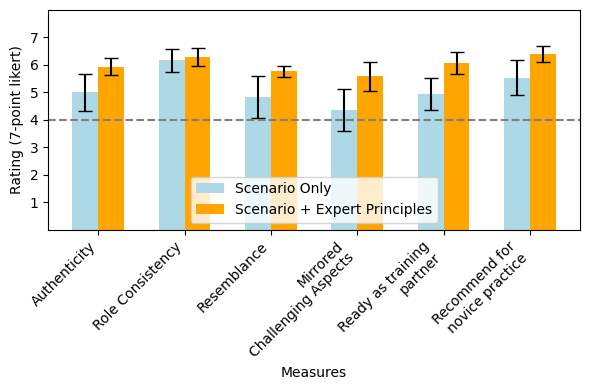
\includegraphics[width=\columnwidth]{figures/creatorstudy-comparison.png}
    \caption{Creator ratings of simulated helpseekers. \emph{Scenario+Expert Principles} shows a significantly higher score than \emph{Scenario Only} on authenticity ($\mu_2=5.9$, $\mu_1=5.0$, **, $d=.66$), resemblance to past case ($\mu_2=5.8$, $\mu_1=4.8$, *, $d=.59$), mirroring challenging aspects ($\mu_2=5.6$, $\mu_1=4.4$, *, $d=.76$), readiness as training partner ($\mu_2=6.0$, $\mu_1=4.9$, ***, $d=.93$), and recommendation for novices ($\mu_2=6.4$, $\mu_1=5.5$, **, $d=.66$). No difference was found for role consistency ($\mu_2=6.3$, $\mu_1=6.2$, $d=.13$). (***:$p<.001$, **:$p<0.01$, *:$p<0.05$. $d$: Cohen's $d$ calculated by dividing by $\sigma_1$ of control group~\cite{lakens2013calculating}.}
    \label{fig:creatorstudy-comparison}
\end{figure}

  
\subsection{Creator Perceptions of Scenario-Only vs Scenario+ExpertPrinciple Roleplay}
% Quantitative - Authenticity, Challenge, Readiness

We investigate how counseling expert principles improve the faithfulness and usefulness of the LLM-simulated help seekers by analyzing creators' ratings of their {\em Scenario-Only} and {\em Scenario-ExpertPrinciple bots}.  Figure~\ref{fig:creatorstudy-comparison} shows the results from conducting paired t-tests and computing effect sizes. The simulated helpseekers shaped by \textit{Scenario+ExpertPrinciples} were rated significantly higher on all measures, except for role consistency for which both bots score highly.
% After counselors have the chance to add their principles to shape their bot's behavior, they perceive the bot to be more authentic, better resemble their past scenario, and more closely mirror the challenging aspects of their scenario. Additionally, creators think it is more ready to be used as a training partner and is more highly recommended for novices to practice with. 

\textbf{Similar Role Consistency:} For both bots, creators found the bot's responses to stay in their role as both were detailed and accurate in reflecting the scenarios described, in regards to the emotional state, attitudes, and the nature of the problems faced. This is a comment on the effectiveness of the GPT-4 dialogue-simulation prompt in generating consistent responses that expand upon the details of the help-seeker scenario contributed by each counselor.

\textbf{Weaknesses of Scenario-Only:} 
Counselors commented on the limitations of the simulated help-seeker powered by the \textit{Scenario-Only} dialogue simulation in Part I. They mentioned it \textbf{lacked the emotional depth}, noting that rather than robotically stating an emotional feeling such as \textit{I feel hopeless}, a realistic helpseeker should display their current emotional state in their manner of speech. 
 Several participants said the bot was \textbf{too articulate and forthcoming} when describing feelings or problems, which is not typically the case for helps-seekers; in real-conversations, helpseekers can have disorganized thoughts, and getting them to describe issues or feelings can be \textit{"as challenging as pulling teeth"}. Participants felt that the bot was \textbf{too cooperative} and too willing to engage in problem-solving and accept help compared to real-life counseling interactions. Notably, some counselors explicitly wrote in their scenario behavioral traits such as \textit{"not talkative"} and \textit{"reluctant"}; yet, they noticed that the Scenario-only simulation struggled to properly exhibit and adhere to these stated behaviors.

% \textbf{Impact of Adding Expert-Principles:} 


\begin{table*}
    \centering
    \begin{tabular}{|l|l|l|} \hline 
         Common Principles&  make responses concise and direct (12 bots)&  \\ \hline 
         &  Theme B&  Example B\\ \hline 
         &  Theme C&  Example C\\ \hline 
         Rare Principles&  Theme D&  Example D\\ \hline 
         &  Theme E&  Example E\\ \hline 
         &  Theme F&  \\ \hline
    \end{tabular}
    \caption{Qualitative Analysis of Principles and Representative Examples}
    \label{tab:my_label}
\end{table*}
\subsection{Creating Principles with Roleplay-doh}
\textit{\textbf{Analysis of Principles:}} Across the 17 help-seeker bots, 85 total principles were created (for a single bot, min=2, max=9, median=5). Two authors did qualitative coding of these principles following a thematic analysis approach~\cite{braun2006thematicanalysis}, where the initial code set came from the themes from the post-survey with creators and was expanded upon during the coding process. 

% What principles were created
To create more authentic and faithful roleplays of the challenging scenario, counselors added principles for the simulated patient to describe emotions in more depth (9 bots), and display their emotions rather than directly saying the emotion they are feeling (4 bots). Principles about providing specific examples or detailed accounts of an experience or emotion (5 bots) could afford counselors the opportunity to use \textit{empathy} or \textit{reflection} skills.

Principles were added for saying less about one's problems and feelings all at once (8 bots), with explicit instructions to allow the listener to naturally ask followups (6 bots). Principles stated that bot responses should stay concise and direct in their descriptions (12 bots) and communicate in a less articulate and more casual style (3 bots). 
Several bots were given principles to be less self-aware of their problems (3 bots) and to start by not seeking solutions but just sharing feelings and experiences (2 bots).  
% Counselor's corrected the bot from being so forthcoming by instructing it to not suggest its own solutions 
Principles were added for the help-seeker bots to share negative outcomes of their past attempts to show a sense of defeat (3 bots); relatedly, bots were also instructed to express hesitancy on whether a suggested coping strategy would work for them (8 bots). Some principles sowed a general mistrust towards the counselor and aimed to place a strain on the therapeutic alliance from the start (4 bots); such principles made the bot more resistant to the stages of counseling, such as sharing feelings or problem-solving. 

% Qualitative Comparison, along these dimensions
While there were many overlaps in the kinds of principles defined, we observed several groupings of principles that appeared like opposites of one another. For example, the call for being disorganized in one's thoughts and exhibiting multiple unrelated or conflicting thoughts (4 bots) contrasts calls to make responses concise and direct (12 bots).  Several counselors added principles to make the help-seeker bot proactively ask for advice, such as how to find effective coping mechanisms for an ongoing struggle or insights on how to change their situation (6 bots); nonetheless, other counselors added an opposing principle to not seek out solutions but rather just share their thoughts and feelings (2 bots). Looking further, these two principles are not incompatible: the need to be heard and share one's emotions or experiences could be prioritized before seeking solutions, but ultimately a person who is motivated to change may seek additional advice on how to do so given current attempts or limitations. 
Our results underscore how different behaviors can manifest in the diversity of help-seekers; different principles are needed to capture the variations in help-seeker behavior, which can challenge the notion that a single set of principles can define a single authentic help-seeker bot. 

% What statistics, and patterns of use arose?

% What are creator's feedback on using the tool to create principles"
\textbf{Tool User Experience:} Results from the tool use questionnaire indicated that counseling experts found Roleplay-doh to be helpful for writing rules that \textbf{effectively guided} the bot to recreate their past case ($\mu=6.23$, $\sigma=0.75$). 
Using the tool, participants perceived it to be \textbf{easy} to convert their thoughts and feedback on the bot's behavior into rules for it to follow ($\mu=6.29$, $\sigma=.84$). Participants also felt they could quickly and \textbf{efficiently} write rules for the bot ($\mu=6.41$, $\sigma=.87$). Finally, participants felt writing principles in Roleplay-doh did not require much \textbf{mental demand} ($\mu=3.23$, $\sigma=1.75$). 
% Although we did not directly compare a version of Roleplay-doh with and without its principle elicitation features, since an ablation study of Roleplay-doh's principle elicitation features was not in scope, these summary statistics are similar to what ~\citet{petridis2023constitutionmaker}'s participants report. 
These ratings of the tool are similar to what ~\citet{petridis2023constitutionmaker}'s participants report. 
Participants elaborated on this positive sentiment, describing how the tools \emph{"translated"} and \emph{"organized"} their thoughts into rules, so they \emph{"didn't have to word it perfectly, [they] just had to say the general idea of what [they] meant."} Together, these results suggest that Roleplay-doh's features for converting feedback into clear principles to follow are helpful for counseling experts to faithfully recreate helpseeker behaviors with LLM-powered simulations.      
% another quote: impressed by the ease at which the tool interpreted my feedback and turned it into a principle that the Member Bot followed. 

% Any critiques or wishes for improvement on tool?
% Any patterns which led people to kind of struggle to shape/steer behavior? 
\if 0
- feedback to principle to alignment analysis
- how many cases where principles had to be edited? 
- or where there were double principles, to kind of get at the same theme? [but also where we can separate out double-click of principles based on time-stamp?]
- or cases where principle adherance was still an issue? [I think this is out of scope for this section, better handled by Ananjan's self critique analysis]
- 1 case where there were bugs in the principle elictation, so they were forced to write.  To aid, they could talk aloud and discuss with experimenter (first author) to help them articulate feedback into a principle.
\fi